\section{Amantadine-like DARPin-F10 modelling}
\label{appendix:amantadineDarpin}

\begin{figure}[H]
\begin{center}
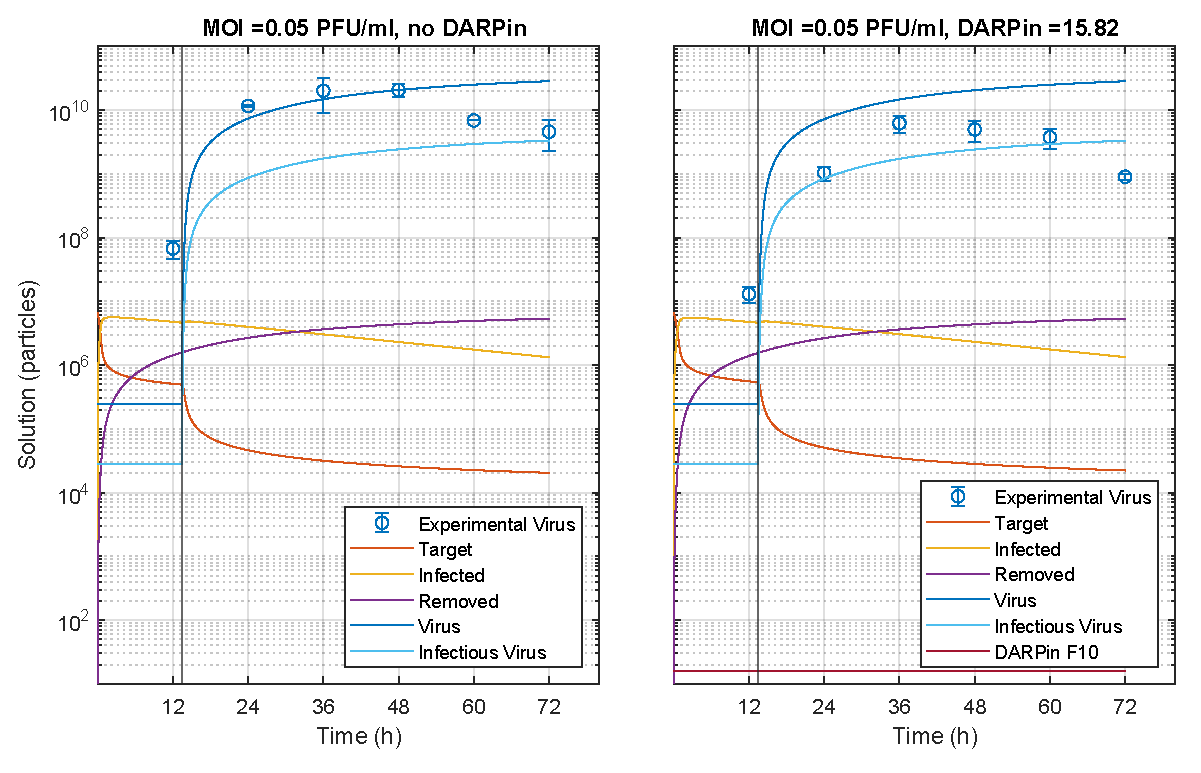
\includegraphics[width=0.6\textwidth, trim={0cm 0cm 0cm 0cm}, clip]{D_chapters/3_DARPinModels/2_DARPinInfection/comparisonModelTHillIRVViDelayMOI0.072135DARPin15.816AsymmetricDarpinMyosinInhibitor.pdf}
\caption[Amantadine-like DARPin-F10 for MOI = 0.05 PFU/ml and $F_{effective}$ = 15.82]{Amantadine-like DARPin-F10 influence on the influenza infection for MOI = 0.05 PFU/ml and relative DARPin-F10 $[F]_{effective}$ = 15.82, calculated based on uncoating experiment. Experimental data is normalized to the simulated virus production value at 48h for no DARPin case.}
\label{figure:amantadineLikeF15}
\end{center}
\end{figure}

\begin{figure}[H]
\begin{center}
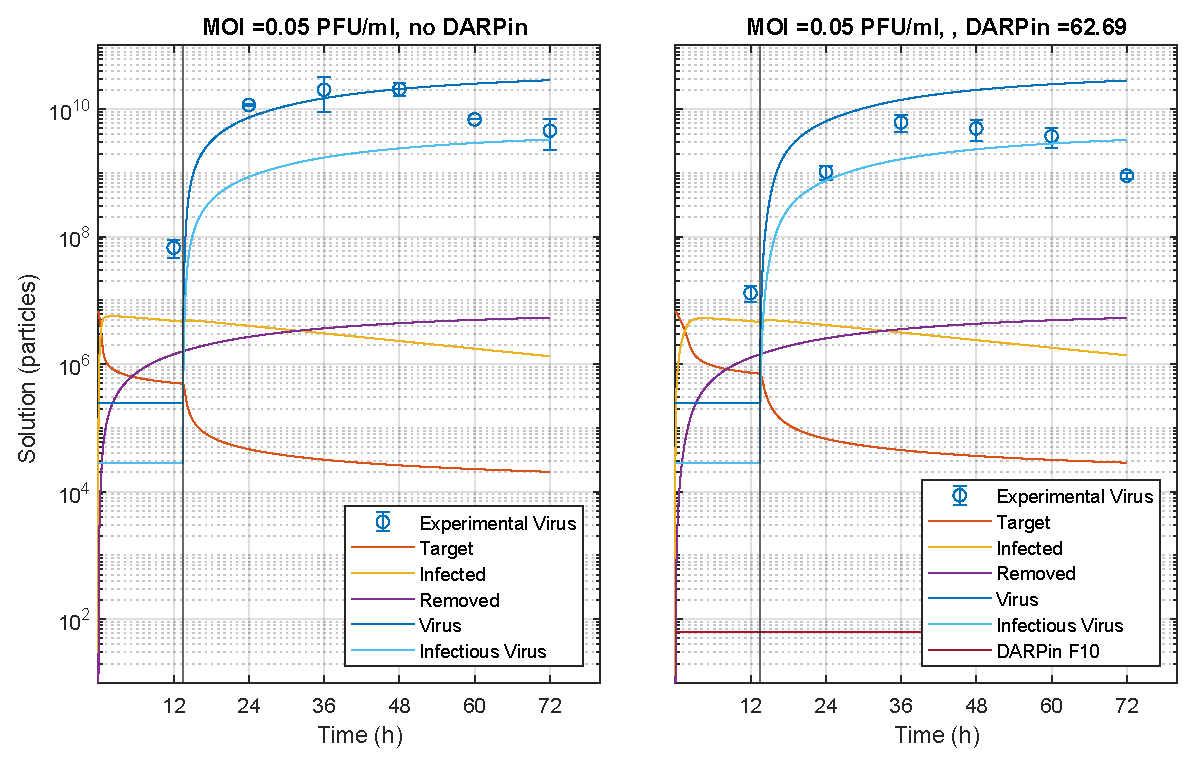
\includegraphics[width=0.6\textwidth, trim={0cm 0cm 0cm 0cm}, clip]{D_chapters/3_DARPinModels/2_DARPinInfection/comparisonModelTHillIRVViDelayMOI0.072135DARPin62.6898AsymmetricDarpinMyosinInhibitor.pdf}
\caption[Amantadine-like DARPin-F10 for MOI = 0.05 PFU/ml and $F_{effective}$ = 62.69]{Amantadine-like DARPin-F10 influence on the influenza infection for MOI = 0.05 PFU/ml and relative DARPin-F10 $[F]_{effective}$ = 62.69, calculated based on viral growth curves at MOI = 0.05 PFU/ml. Experimental data is normalized to  the simulated virus production value at 48h for no DARPin case.}
\label{figure:amantadineLikeF62}
\end{center}
\end{figure}

\section{Neuraminidase inhibitor-like DARPin-F10 modelling}
\label{appendix:neuraminidaseInhibitorDarpin}
\begin{figure}[H]
\begin{center}
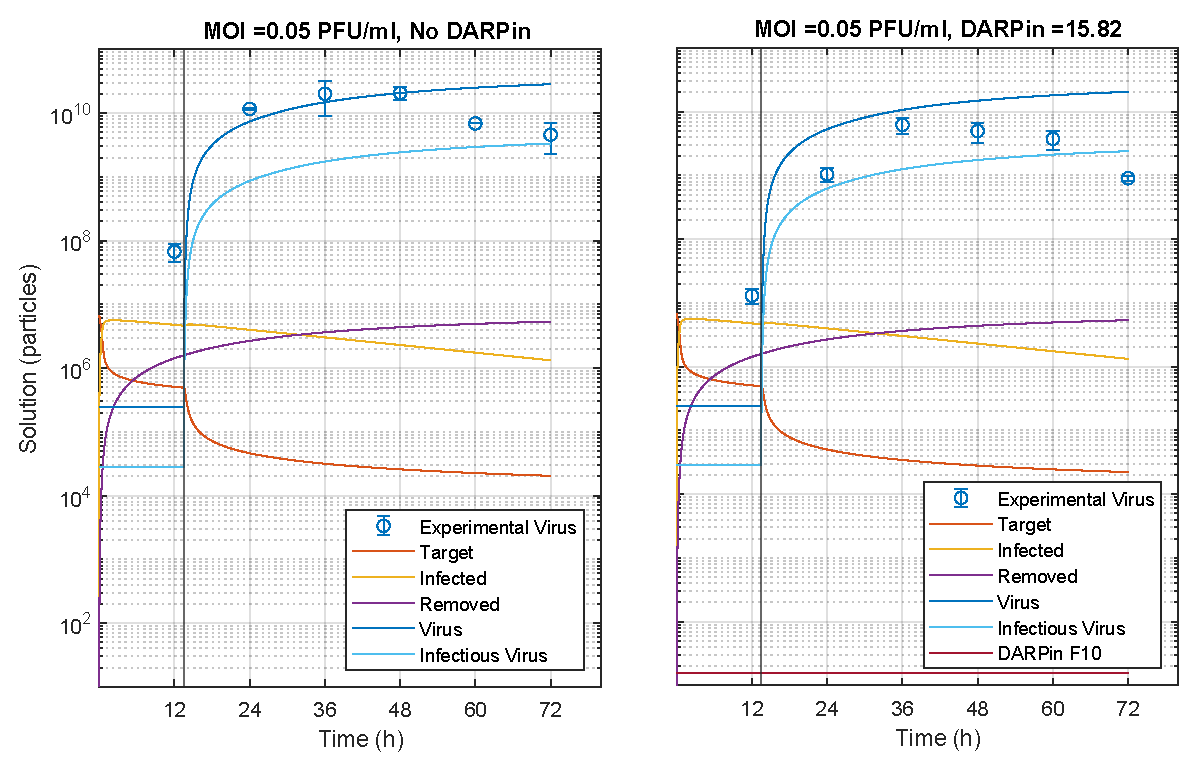
\includegraphics[width=0.6\textwidth, trim={0cm 0cm 0cm 0cm}, clip]{D_chapters/3_DARPinModels/2_DARPinProduction/comparisonModelTHillIRVViDelayMOI0.072135DARPin15.816AsymmetricDarpinMyosinInhibitor.pdf}
\caption[Neuraminidase inhibitor-like DARPin-F10 for MOI = 0.05 PFU/ml and $F_{effective}$ = 15.82]{Neuraminidase inhibitor-like DARPin-F10 influence on the influenza infection for MOI = 0.05 PFU/ml and relative DARPin-F10 $[F]_{effective}$ = 15.82, calculated based on uncoating experiment. Experimental data is normalized to  the simulated virus production value at 48h for no DARPin case.}
\label{figure:neuraminidaseInhibitorLikeF15}
\end{center}
\end{figure}

\begin{figure}[H]
\begin{center}
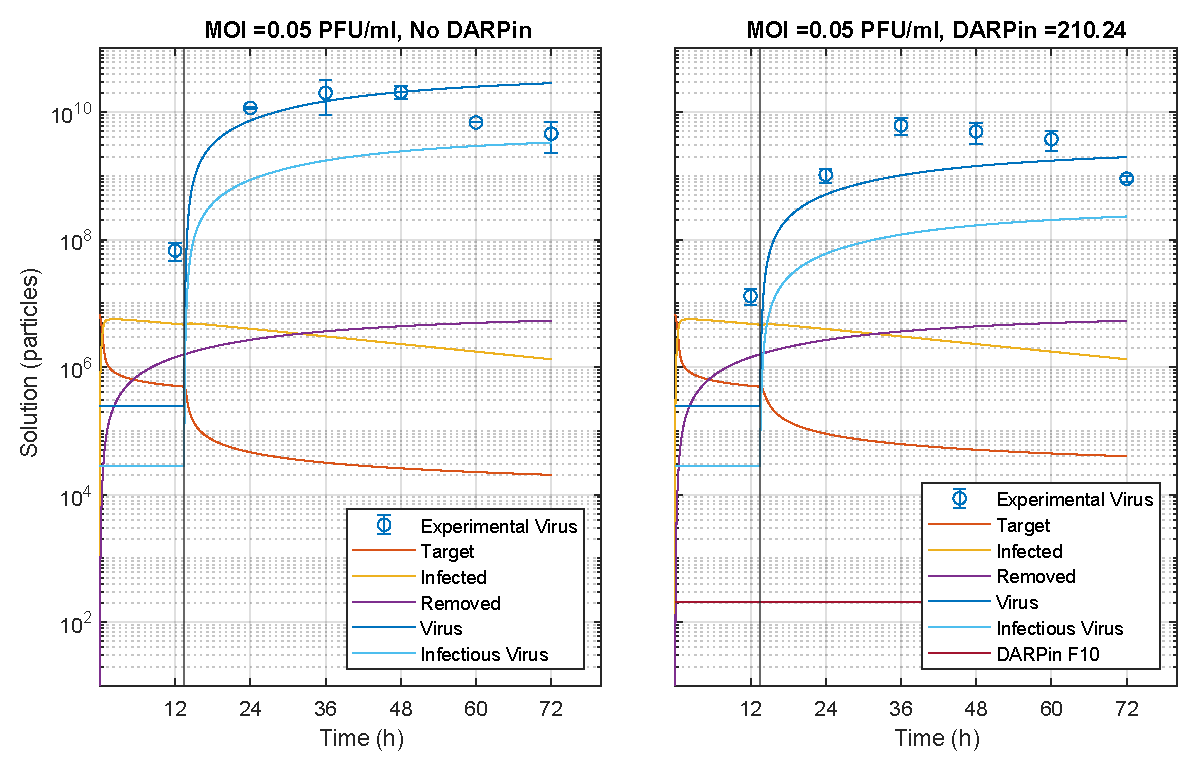
\includegraphics[width=0.6\textwidth, trim={0cm 0cm 0cm 0cm}, clip]{D_chapters/3_DARPinModels/2_DARPinProduction/comparisonModelTHillIRVViDelayMOI0.072135DARPin210.236AsymmetricDarpinMyosinInhibitor.pdf}
\caption[Neuraminidase inhibitor-like DARPin-F10 for MOI = 0.05 PFU/ml and $F_{effective}$ = 210.24]{Neuraminidase inhibitor-like DARPin-F10 influence on the influenza infection for MOI = 0.05 PFU/ml and relative DARPin-F10 $[F]_{effective}$ = 210.24, calculated based on viral growth curves at MOI = 10 PFU/ml. Experimental data is normalized to  the simulated virus production value at 48h for no DARPin case.}
\label{figure:neuraminidaseInhibitorLikeF210}
\end{center}
\end{figure}